\documentclass[letter, USenglish, 11pt, subfigure]{article}
\usepackage[margin=1in]{geometry}
\usepackage{pdfpages}
\newcommand*{\ATLASLATEXPATH}{./}
\usepackage{\ATLASLATEXPATH atlaspackage}
\usepackage{\ATLASLATEXPATH atlasbiblatex}
\usepackage{\ATLASLATEXPATH atlasphysics}
\newcommand{\mm}{\ensuremath{\mu^{+}\mu^{-}}}
\newcommand{\bsmm}{\ensuremath{\Bs\to\mm}}
\newcommand{\bdmm}{\ensuremath{\Bd\to\mm}}

\addbibresource{proposal_WHopkins.bib}
\pagestyle{headings}

\title{Machine-Learning-Driven New Physics Searches at the Large Hadron Collider}
\author{Walter Hopkins, Assistant Physicist\\
}
\date{}

\begin{document}
%\pagenumbering{gobble}

\maketitle

\section{Budget justification}

\subsection{Senior/Key Person}
\label{subsec:keyPerson}
The PI is the only senior person that will be funded. The PI will be funded at an average of 0.57 FTE. For the first two budget periods the PI will be funded at 0.6-0.7 FTE to aid in the start up of the proposed work while for the remainder of the proposed work the PI will be funded at 0.5 FTE. Table~\ref{tab:yearlyBudget} shows the breakdown of the PIs FTE for each budget period.

\begin{table}[!htpb]
  \begin{center}
    \caption{Budget for each period. Fringe/indirects are not included.}
      \label{tab:yearlyBudget}
  %\scriptsize
  \begin{tabular}{lrrrr|rrrr}
\hline
 & \multicolumn{4}{c|}{Scientific} & \multicolumn{4}{c}{Postdoctoral} \\
{} & Months & Salary & Fringe & Totals & Months & Salary & Fringe & Totals \\
\hline
Period 1 &       8.2 &    \$121,622 &      \$36,486 &  \$158,108 &           13.0 &          \$75,993 &           \$22,798 &        \$98,791 \\
Period 2 &       6.2 &     \$96,072 &      \$28,821 &  \$124,893 &           20.0 &         \$122,225 &           \$36,667 &       \$158,892 \\
Period 3 &       6.0 &    \$105,602 &      \$31,681 &  \$137,283 &           30.0 &         \$191,015 &           \$57,305 &       \$248,320 \\
Period 4 &       6.0 &    \$109,687 &      \$32,906 &  \$142,593 &           24.0 &         \$159,220 &           \$47,766 &       \$206,986 \\
Period 5 &       6.0 &    \$113,932 &      \$34,179 &  \$148,111 &           15.0 &         \$103,701 &           \$31,110 &       \$134,811 \\
\hline
Total    &      32.4 &    \$546,915 &     \$164,073 &  \$710,988 &          102.0 &         \$652,154 &          \$195,646 &       \$847,800 \\
\hline
\end{tabular}

  \end{center}
\end{table}

\subsection{Other Personnel}
\label{subsec:personnel}
Other personnel will include an average of 1.5 FTE of postdocs. A postdoc, at 1.0 FTE, will be hired seven months into the first budget period. Additional effort during will come from an existing ANL ATLAS group postdoc who will be funded at 0.5 FTE and who will focus on accelerating the computational performance of the ATLAS detector simulation. The contract of the first 1.0 FTE postdoc (hired in budget period 1) will end in budget period 4. A new postdoc at the same level will be hired (at the beginning of budget period 3) in time to replace this effort and will be funded until the end of budget period 5. The newly-hired postdocs will both work on the search strategy and simulation projects (each at 0.5 FTE resulting in 1.0 FTE per subtask). Table~\ref{tab:yearlyBudget} shows the breakdown of the postdoc FTEs for each budget period.
\clearpage
\subsection{Equipment}
\label{subsec:Equipment}
The request equipment is a GPU workstation at the cost of \$21,000 (not including indirect costs). The workstation is needed to for fast development and testing of ML algorithms before they are deployed on a larger scale at ALCF resources. Specifically, the graphical processing units (GPUs) are essential for ML tasks such as training and early optimization studies. To enable the testing of scaling, which is essential for running on large HPC resources, the workstation would contain at least two NVIDIA GPU cards. The GPU cards should contain at least V100 cores but the exact type of core will be decided closer to the purchase date. 

\subsection{Travel}
\label{subsec:travel}
Travel will consist of trips to CERN for the PI and postdocs. Based on previous experience, travel to CERN costs \$3000 per trip. About two trips per year and per person will be made to CERN. These trips will be to attend the ATLAS Physics and Performance (P\&P) weeks and the Software and Computing (S\&C) weeks which are held multiple times a year. The P\&P weeks are essential in communicating with ATLAS collaborators on the use of clustering for the ongoing and future pMSSM scans. The S\&C weeks host broader simulation meetings which will be used by the PI's team to collaborate on enhancing the computational speed of detector simulations.

In addition to trips to CERN, three (for the 1.5 postdocs and the PI combined) domestic trips to conferences to highlight results are foreseen every two years. Based on previous experience, these trips cost \$1500. Table~\ref{tab:yearlyTravelBudget} shows the breakdown of travel costs for each budget period. Examples conferences were the new physics search results can be shown are SUSY or ICHEP. These are international conferences that can occur anywhere in the world but the ones that will be domestic will be chosen. For the detector simulation work conferences such as CHEP and ACAT will be considered. These trips are planned for budget period 2, 3 and 5. Budget period 2 will include one trip for the PI and one for the 0.5 FTE ATLAS postdoc to highlight the early detector simulation results based on simplified geometries. Budget period 3 will include one trip for the PI and two trips for the 2.0 FTE postdoc that were hired to work solely on the proposed work. These trips will be to show the results of the pMSSM interpretation and detector simulations with more complex geometries. Finally, budget period 5 will include one trip for the PI, one for the 1.0 FTE postdoc, and finally one for the 0.5 FTE ATLAS postdoc. These trips are meant to share the results of the completed new physics search based on the ML algorithm and early ATLAS simulation results. 

\begin{table}[!htpb]
  \begin{center}  
    \caption{Travel budget and trips per period. Indirect costs are not included.}
    \label{tab:yearlyTravelBudget}
  \begin{tabular}{lrrr}
\hline
{} &  Domestic trips &  International trips & Travel Funds \\
\hline
Budget period 1 &               0 &                    2 &       \$6,000 \\
Budget period 2 &               2 &                    5 &      \$18,000 \\
Budget period 3 &               3 &                    6 &      \$22,500 \\
Budget period 4 &               0 &                    7 &      \$21,000 \\
Budget period 5 &               3 &                    4 &      \$16,500 \\
\hline
\end{tabular}

  \end{center}
\end{table}

\subsection{Participant/Trainee Support Costs}
\label{subsec:trainee}
Not applicable.

\subsection{Other Direct Costs}
\label{subsec:otherDirects}
There are no other direct costs other than the personnel, equipment, and travel costs listed above.

\subsection{Direct Costs}
\label{subsec:directs}
The total direct costs are \$1,663,788 of which \$1,558,788 is in salaries, \$21,000 is for equipment, and \$84,000 is for travel.

\subsection{Other Indirect Costs}
\label{subsec:otherIndirects}
There are two indirect rates one for M\&S/travel and one for personnel. The total indirect costs per budget period are shown in Table~\ref{tab:indirects}.

\begin{table}[!htpb]
  \begin{center}  
    \caption{Indirect costs per budget period.}
      \label{tab:indirects}
  \begin{tabular}{lrr}
\hline
{} & Indirect costs    \\
  \hline
  Budget period 1 &         \$139,873      \\
  Budget period 2 &       \$152,000     \\
  Budget period 3 &         \$206,118      \\
  Budget period 4 &         \$186,990     \\
  Budget period 5 &        \$151,231     \\\hline
  Total           &             \$836,212  \\
  \hline
\end{tabular}

  \end{center}
\end{table}

\subsection{Total Direct and Indirect Costs}
\label{subsec:totalCosts}
The total cost of this proposal is \$2,500,000. The direct, indirect, and total cost per budget period can be found in Table~\ref{tab:total}.

\begin{table}[!htpb]
  \begin{center}  
    \caption{Direct and indirect costs per budget period.}
      \label{tab:total}
  \begin{tabular}{llll}
\hline
{} &   Direct costs & Indirect costs &     Total cost \\
\hline
Budget period 1 &    \$283,899 &     \$139,873 &    \$423,772 \\
Budget period 2 &    \$301,785 &     \$152,000 &    \$453,785 \\
Budget period 3 &    \$408,103 &     \$206,118 &    \$614,221 \\
Budget period 4 &    \$370,579 &     \$186,990 &    \$557,569 \\
Budget period 5 &    \$299,422 &     \$151,231 &    \$450,653 \\\hline
Total           &  \$1,663,788 &           \$836,212 &  \$2,500,000 \\
\hline
\end{tabular}

  \end{center}
\end{table}
\clearpage

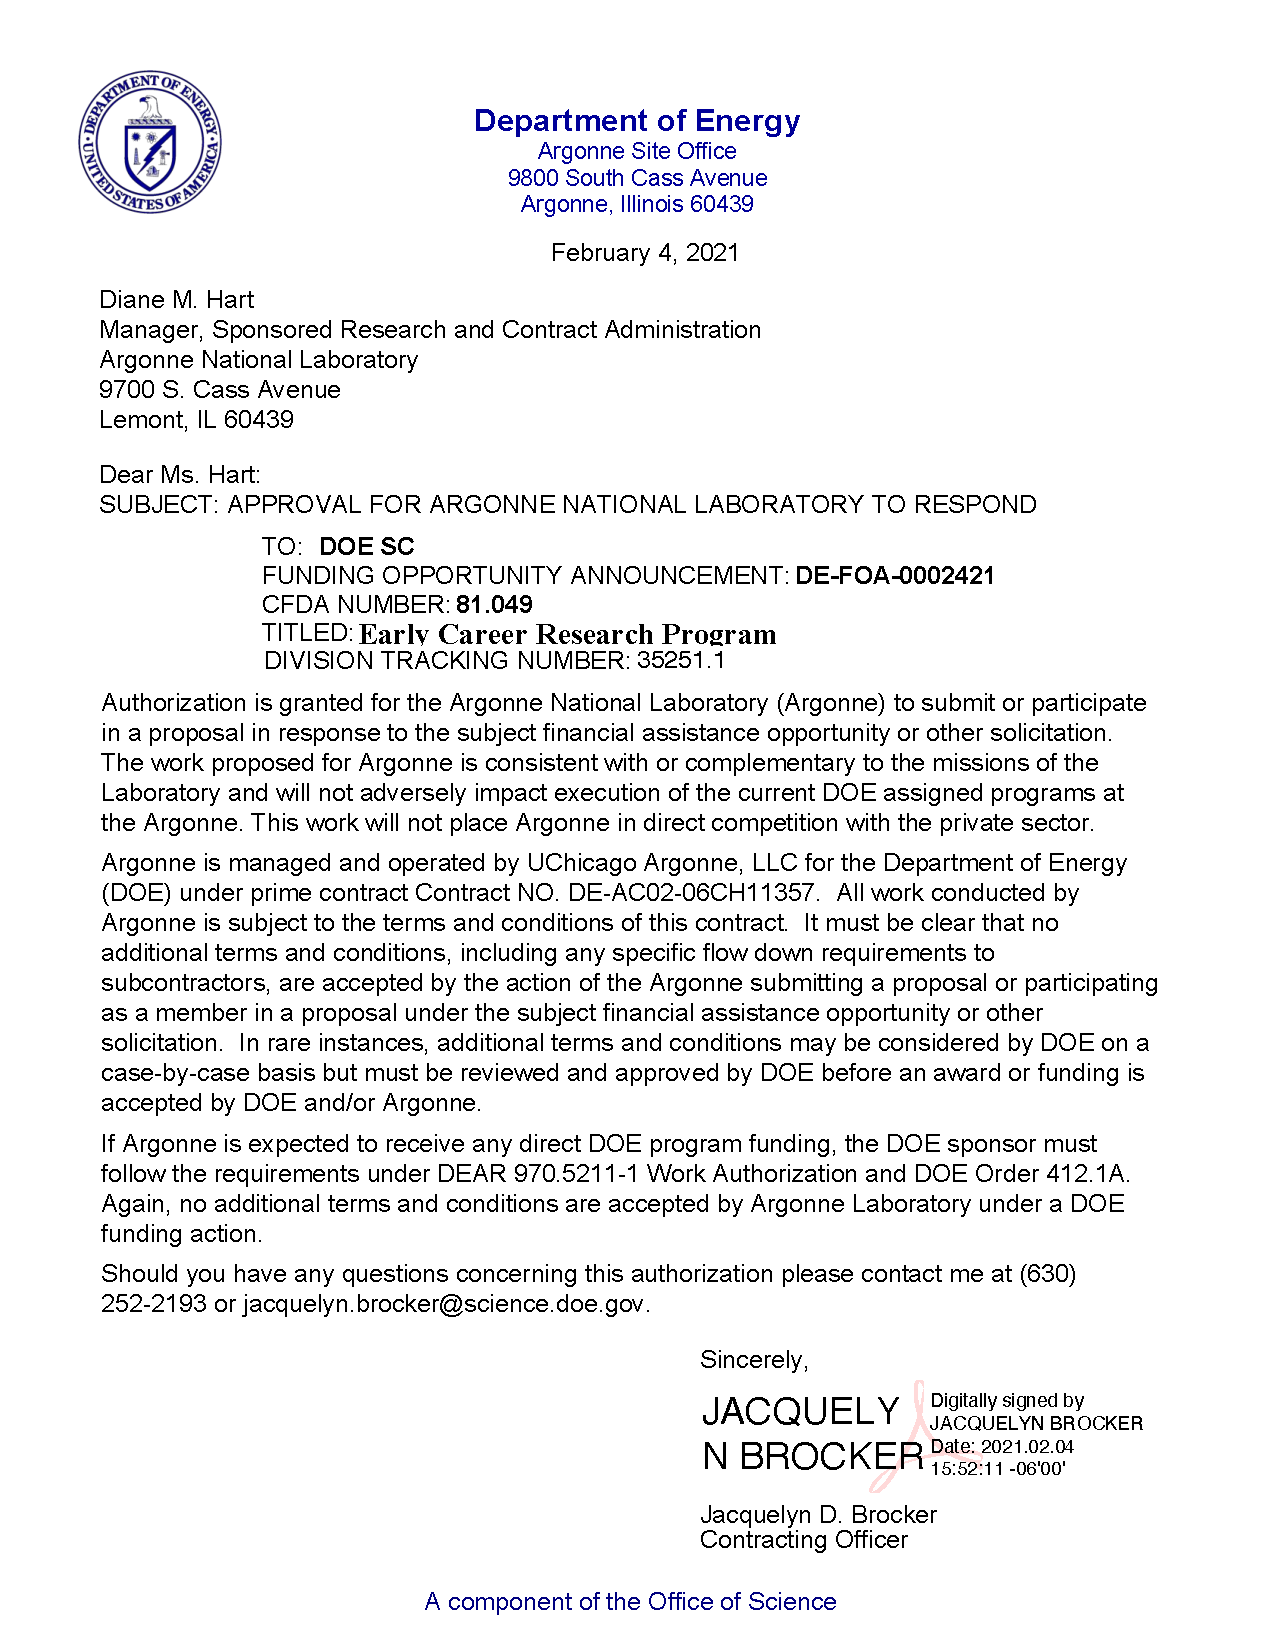
\includepdf{DOE_CO_Approval_Letter_whopkins}

\end{document}

